\chapter{Home Automation}

Home automation, also known as domotics, has been a recurrent topic in Computer Science that
has become a reality in the last decades, thanks to the growth and decrease in the price of embedded
systems and wireless technologies, that have permitted to create distributed systems, the heart of this technology.

\bigskip
In this chapter, I am going to analyze this technology and its current state, including its implementation in commercial
products.

\section{What is home automation?}

Although science fiction has represented the idea of smart houses since the past century, including in them
an intelligence able to respond to all the dweller’s needs and desires, it has never felt as close to real world as today.

\bigskip
The basic idea of home automation is to employ sensors and control systems to monitor a dwelling, and accordingly 
adjust the various mechanisms that provide heat, ventilation, lighting, and other services. By more closely tuning the 
dwelling’s mechanical systems to the dweller’s needs, the automated "intelligent" home can provide a safer, more 
comfortable, and more economical dwelling.\cite{smarthouse98} For example, the automated system can determine 
the intensity and direction of the sunlight, and adequate the house according to its condition (which would include
closing the blinds and adjusting the air conditioner).

\bigskip
Unlike many may think, we don't actually need a very modern house, since advanced systems can be perfectly integrated 
in older, traditional buildings. This fact makes domotics a real possibility in every situation. In fact, the number of home 
automation systems installed in Europe is expected to reach around 29 million by 2019.\cite{statistaInstalled}

\begin{figure}
	\centering
	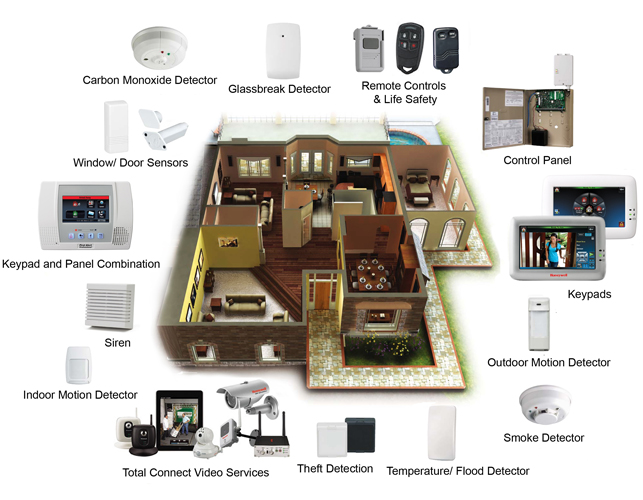
\includegraphics[width=0.9\textwidth]{images/Chapter_02/security.jpg}
	\caption{Example of a smart home with security-oriented devices}
	\label{fig:security-in-smarthome}
\end{figure}

\bigskip
There is not an exact point where we can set the beginning of the domotics as a real concept, but during the last century
there has been some remarkable efforts, and even before. In 1898, Nikola Tesla created a wireless control for a toy boat, 
the first of its kind \cite{betanewsHistory}. That marks the beginning of wireless technologies, one of the fundamental
parts of Home Automation. 

\bigskip
In 1975, after lots of appearances of the idea of home automation in films, the first general purpose home automation
technology, called X10, was developed. X10 defines a protocol for communication between electrical devices, which uses power
line wiring for signaling and control, where the signals involve brief radio frequency bursts representing digital information.
Therefore, it also defines a wireless radio based protocol. Surprisingly, the X10 technology is still widely used and available,
with millions of units in use worldwide.

\bigskip
However, it was not until 1984 that the word Smart Home appeared, invented by the \textit{American Association of House
Builders}. After that, different inventions rapidly followed one another, with devices such as\\ \textit{The Clapper} (which 
was operated through sound, like a clap or a bark) and interest from the biggest technological companies, like Microsoft.

\begin{figure}
	\centering
	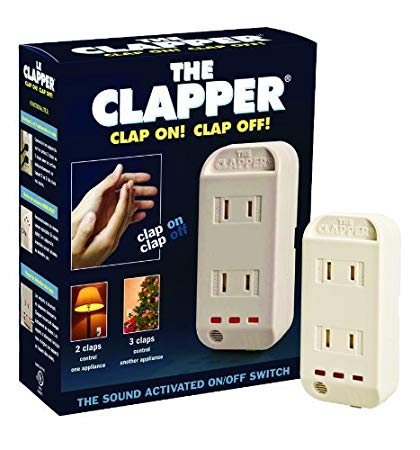
\includegraphics[width=0.5\textwidth]{images/Chapter_02/the-clapper.jpg}
	\caption{The Clapper, a sound-activated switch}
	\label{fig:the-clapper}
\end{figure}

\bigskip
Home Automation has not stopped gaining ground on our homes and now it is experiencing one of the best moments
in its lifetime, with the unstoppable growth of the Internet of Things (IoT) and the simultaneous development of Artificial 
Intelligence for the general public, with the biggest companies, like Google and Apple, investing millions of dollars on it.
Devices like Amazon Echo and Google Home, or assistants like Siri, Cortana, Google Assistant and Amazon Alexa are a 
good representative of this trend. I will talk in depth about them in the following sections.

\bigskip
We have always imagined that Smart Homes would bring us a whole world of benefits. And that is partly true, but
they have ended up offering benefits that no one could imagine some decades before, when matters such as energy
savings were not as important as today. These benefits are responsible for their increasing popularity, and they can be 
summarized in the following points:

\begin{itemize}
	\item \textbf{Control anywhere:} Smart Homes can be completely controlled anywhere in the world from smart phones or
	other devices with Internet connection, so we can know the status of our devices at any time. That would allow us, for
	example, to stop worrying when staging out of home thinking if we have left the air conditioning on.
	\item \textbf{Safety:}
\end{itemize}

What has made so popular the home automation is the broad range of benefits that it offers to their users.


